\chapter{Proposals}
\label{ch_proposals}

\section{API}

A C API is preferred as it is highly portable and permits rapid integration with other programming languages and applications.


\subsection{Creation}

\begin{itemize}
\item The library will use a structure to store all of the parameters related to a single instance of SAFEcrypto.

\begin{verbatim}
      extern safecrypto *safecrypto_create(const char *algorithm);
\end{verbatim}

\item This structure must be created for a particular algorithm using a human readable string identifier.
\item If the structure cannot be created a NULL pointer is returned which the user must check for.
\item A destruct function is used to free all resources allocated to the SAFEcrypto structure and all internal memory resources.
\end{itemize}

\begin{verbatim}
    extern int32_t safecrypto_destroy(safecrypto *sc);
\end{verbatim}


\subsection{Debug Printing}

\begin{itemize}
\item Macros should be provided to allow users to insert arbitrary print statements that will be removed during compilation of a released library.
\item Debug macros should be multi-level to provide a hierarchy of debug statements to improve the efficiency of bug finding.
\item The debug logging facility should be thread-safe to allow its use in those algorithms which make use of concurrency.
\item The debug logging facility should print to a user specified file with a default name.
\item Variadic print functions will be used that provide indentical functional to \textit{printf~()}:
\end{itemize}

\vspace{1em}
\textit{Example use:}

\indent\begin{verbatim}
    int *p = NULL;
    …

    if (p == NULL) {
        SC_LOG_ERROR(sc, SC_NULL_PTR);
        return SC_FUNC_FAILURE;
    }
\end{verbatim}


\subsection{Error Queue}

\begin{itemize}
\item An error queue facility similar to that used by OpenSSL will be used:

\begin{verbatim}
    extern uint32_t safecrypto_err_get_error(safecrypto *sc);
    extern uint32_t safecrypto_err_peek_error(safecrypto *sc);
    extern uint32_t safecrypto_err_get_error_line(safecrypto *sc,
        const char **file, int32_t *line);
    extern uint32_t safecrypto_err_peek_error_line(safecrypto *sc,
        const char **file, int32_t *line);
    extern void safecrypto_err_clear_error(safecrypto *sc);
\end{verbatim}

\item An error message including an error code, file name and line number will be buffered in a finite length queue of errors.
\item If the queue is full new errors will be discarded such that the possible root cause of an issue will remain in the buffer.
\item Error messages will automatically utilise the debug printing facility if it is enabled.
\item It is the user’s responsibility to manage the error queue.
\end{itemize}

\subsection{Parameters}

\begin{itemize}
\item Store all parameters as arrays of length 1 or greater using dynamic memory.
\item All parameters will have a unique human readable name used for identification.
\item All parameters are stored in some form of linked list with nodes composed of struct’s containing all necessary details (name, type, length and a void* pointer to the array of data).

\begin{verbatim}
    typedef enum sc_param_type {
        SC_PARAM_UINT8 = 0,
        SC_PARAM_UINT16,
        SC_PARAM_UINT32,
        SC_PARAM_INT8,
        SC_PARAM_INT16,
        SC_PARAM_INT32,
        SC_PARAM_FLOAT,
        SC_PARAM_DOUBLE,
    } sc_param_type_e;

    typedef struct sc_param {
        char name[SC_MAX_NAME_LEN];
        safecrypto_param_type_e type;
        void *value;
        int32_t length;
    } sc_param_t;
\end{verbatim}


\item A simple API function is provided to obtain a pointer to the struct containing the parameter with a specified name:

\begin{verbatim}
    extern safecrypto_param_t *safecrypto_param_get(safecrypto *sc,
        const char *name);
\end{verbatim}

\item Where the name of parameters is unknown, functions are provided to iteratively parse the linked list:

\begin{verbatim}
    extern safecrypto_param_t *safecrypto_param_get_first(safecrypto *sc);
    extern safecrypto_param_t *safecrypto_param_get_next(safecrypto *sc,
        safecrypto_param_t *param);
\end{verbatim}

\item When each allgorithm is initialised it MUST populate the linked list of parameters with an initial set of known good parameters.
\item A helper function is provided to allow parameters for the selected algorithm to be configured according to the minimum number of permitted security bits.
\end{itemize}

\vspace{1em}
\textit{Example usage:}

\indent\begin{verbatim}
    safecrypto *sc = safecrypto_create(“Algorithm A”);
    …

    // List all parameters
    safecrypto_param_t *param = safecrypto_param_get_first(sc);
    while (param != NULL ) {
        // Print the parameter details
        printf(“Parameter %s has %d elements:\n”, param->name, param->length);
        switch (param->type)
        {
        case SC_PARAM_UINT8:
            uint8_t *p = (uint8_t *)param->value;
            for (int i=0; i<param->length; i++)
                printf(“%02X ”, (int)(*p++));
            printf(“\n”);
            break;
        case SC_PARAM_UINT16:
        ...
        default:;
        }
        param = safecrypto_param_get_next(sc, param);
    }
\end{verbatim}



\newpage
\section{Dynamic Configuration}

\subsection{Assumptions}

\begin{itemize}
\item The API provides a method that permits arbitrary parameters to be created, modified and used by any algorithm.
\end{itemize}

\subsection{Goals}

\begin{itemize}
\item As algorithms are developed the necessary mathematical and cryptographic functions will be implemented into a library of functions known as the toolbox.
\item The functions within the toolbox will be configurable at compile time to support optimizations for various processor architectures.
\item The toolbox will provide the functionality required to implement more abstract functions, thereby reducing development time and providing a similar platform on which to compare algorithms.
\end{itemize}

\subsection{Proposed Implementation}

\begin{itemize}
\item All functions/classes within the toolbox will be named with the prefix tb to enable their easy identification.
\item An additional prefix will be used to idenify the type of function (e.g.\ prf for pseudo random function, arith for arithmetic functions such as polynomial or matrix manipulation, thread for concurrency functions, etc.)
\item These functions MUST be used where any significant data processing occurs.
\item If functionality offered by the toolbox is not available then it must be implemented within the toolbox if it is believed it can be re-used elsewhere.
\item All toolbox functions MUST be unit tested.
\end{itemize}


\subsection{Algorithms and Toolbox Written in C or C++~?}

\textbf{Advantages of C}
Industry guidelines are easier to prove in C (e.g. SEI CERT, MISRA).
Extreme performance offered by efficient compilers and a well defined C ABI, C++ compilers can miss optimizations if certain language features are used.
Widespread support and portability.
Easier to pick up and understand than C++.

\textbf{Advantages of C++}
OOP leads to better modularisation, testability and code-reuse.
Runtime and compile time polymorphism lends itself to a library that is designed to be highly configurable, negating the need for void* which can hinder compiler optimizations and is difficult to understand and maintain.
Can be used without exceptions, etc.\ to provide better performance.
Arithmetic operations can be implemented as operators rather than function calls to improve the readabiity of code.


\newpage
\section{PRNG Revision 2}

\subsection{Reasons for Revision}

S{\`e}amus' statistical work on RNGs has highlighted some changes that we need to make to the SAFEcrypto RNG to make it more robust, cryptographically secure and follow accepted methodology for a secure RNG in a cryptographic library. A number of additional CSPRNG's may be of interest for further study and/or use within SAFEcrypto. It would also be beneficial to integrate more debug and statistics gathering capabilities into the SAFEcrypto PRNG source code.

\begin{figure}[!h]
\centering
%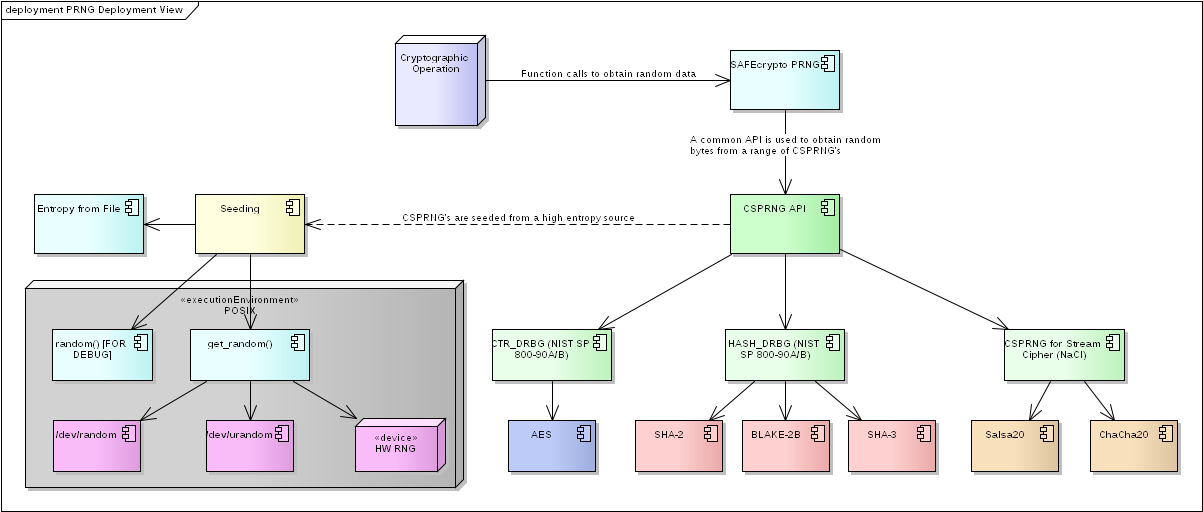
\includegraphics[width=22cm,angle=90]{proposal_prng_version_2.png}
\caption{PRNG deployment view}
\label{fig:prng_proposal}
\end{figure}

\subsection{CSPRNG's Of Interest}

All CSPRNG's will use a common PRNG API to allow them to fill a buffer with \textit{n} bytes of random data. This buffer will then be used to provide all random data for user calls to PRNG functions.

\begin{enumerate}
\item Hash-DRBG - with SHA-2 and SHA-3. \textbf{NOTE: Use NIST HASH\_DRBG test vectors}
\item CTR-DRBG - with AES. \textbf{NOTE: Use NIST AES-CTR test vectors.}
\item Salsa20 CSPRNG - based on the example CSPRNG in NaCl (Bernstein).
\item ChaCha20 CSPRNG - will be replaced with Bernstein's implementation, CSPRNG aspect will use NaCl example.
\item KISS/Mersenne Twister
\item ISAAC64/32
\end{enumerate}

\subsection{Seeding}

All CSPRNG's will be seeded using a user selectable seed source which will include POSIX system \textit{random()}, \textit{\\dev\\random} and \textit{\\dev\\urandom} using POSIX system \textit{getrandom()} calls, and from a pre-generated entropy file for debug and test purposes only. \textbf{NOTE: A correctly configured Linux machine is capable of using \textit{\\dev\\hwrng} to populate \textit{\\dev\\random} and \textit{\\dev\\urandom}. Therefore we shouldn't specifically provide support for HW RNG's.}

The custom functions currently used to seed using \textit{\\dev\\random} and \textit{\\dev\\urandom} will be replaced with the \textit{getrandom()} function. This is because the \textit{getrandom() system call fills the buffer pointed to by buf with up to buflen random bytes.  These bytes can be used to seed user-space random number generators or for cryptographic purposes.} See \url{https://lwn.net/Articles/606141/}.

\subsection{No Wasted Data}

To try and avoid any strange results all generated random bits will be consumed. For example, random bits being drawn from the LSB's of 32-bit \textit{prng\_32()} calls, discarding all but the required LSB's and exposing the RNG to any periodic data from the LSB's of the CSPRNG's.

Therefore a new PRNG function call will be provided, \textit{prng\_var(int n)}, that will allow a user to arbitrarily obtain 1 to 32 random bits.

\subsection{Multithreading}

The PRNG \textbf{MUST} be thread safe as it will be used in multithreaded implementations of the library.


\subsection{Statistics Gathering}

A C struct containing a range of information gathered from an instance of the SAFEcrypto PRNG will be maintained. The information gathered will include the following:

\begin{itemize}
\item Selected source (i.e. \textit{random()}, \textit{\\dev\\random} and \textit{\\dev\\urandom}.)
\item Seed bits generated from the source
\item Selected (CS)PRNG
\item Random bits generated from the (CS)PRNG
\item Total bits consumed
\item Bits consumed from each API call (e.g. \textit{prng\_32(), prng\_8()} etc.)
\end{itemize}

\subsection{Integration Callback API}

It can be argued that if/when the SAFEcrypto library is integrated into another application that an RNG may already be available within that application. Therefore it should be possible to provide an API using callback functions to deliver the same RNG functionality of SAFEcrypto's internal RNG using those already provided by the application.

\textbf{\textit{NOTE: The Callback API will be treated as a feature request with low priority.}}



\section{Multithreading and Hardware Integration}


\subsection{Key Generation}

\begin{algorithm}[H]
\begin{algorithmic}[1]
\Function{BLISS Key Generation}{Key pair (\textbf{A,S}) such that \textbf{AS}$ = q \bmod{2q}$}
\State Choose \textbf{f, g} as uniform polynomials with exactly $d_1 = \lceil{\delta_1 n}\rceil$ entries in ${\pm1}$ and $d_2 = \lceil{\delta_2 n}\rceil$ entries in ${\pm2}$
\State \textbf{S} $= (s_1,s_2)^t \leftarrow ($\textbf{f}$, 2$\textbf{g}$+1)^t$
\If {$N_\kappa ($\textbf{S}$) \ge C^2 \cdot 5 \cdot (\lceil\delta_1 n\rceil + 4 \lceil \delta_2 n \rceil) \cdot \kappa$}
  \State \textbf{restart}
\EndIf
\State $a_q = (2g+1)/$\textbf{f}$ \bmod{q}$ (\textbf{restart} if \textbf{f} is not invertible)
\State \textbf{Output} $(A,S)$ where $A = (2 a_q, q-2) \bmod{2q}$
\EndFunction
\end{algorithmic}
\caption{BLISS Key Generation}
\end{algorithm}


